% Source map (line numbers refer to original activities):
% Practice: book2026-2027/grade11/term_2/1-practice_activities/G11_T2_L1_C3_practice.tex
% Classroom: book2026-2027/grade11/term_2/2-class_activities/G11_T2_L1_C3_classroom_activity.tex
% Worked example boundary: classroom lines 125--269; stop before Guided Example.
% Only prerequisites needed for this example are imported. Sources remain unmodified.
\documentclass[12pt,aspectratio=169]{beamer}
\usepackage[T1]{fontenc}
\usepackage{lmodern}
\usepackage{amsmath,amssymb,array,booktabs,tabularx,tikz,pgfplots}
% Add language support appropriate to the source, if needed.
% Keep this preamble inline in every delivered deck.
\definecolor{GEInk}{HTML}{132A3E}
\definecolor{GETeal}{HTML}{17675E}
\definecolor{GEFooter}{HTML}{EAF2F1}
\setbeamercolor{background canvas}{bg=white}
\setbeamercolor{normal text}{fg=GEInk,bg=white}
\setbeamercolor{structure}{fg=GETeal}
\setbeamercolor{frametitle}{fg=GEInk}
\setbeamercolor{GE footer}{fg=GETeal,bg=GEFooter}
\setbeamerfont{normal text}{family=\sffamily,size=\normalsize}
\setbeamerfont{title}{size=\huge,series=\bfseries}
\setbeamerfont{subtitle}{size=\normalsize,series=\bfseries}
\setbeamerfont{frametitle}{size=\Large,series=\bfseries}
\setbeamerfont{framesubtitle}{size=\normalsize,series=\mdseries}
\setbeamerfont{GE footer}{size=\footnotesize}
\setbeamersize{text margin left=9mm,text margin right=9mm}
\setbeamertemplate{navigation symbols}{}
\setbeamertemplate{headline}{}
\setbeamercovered{invisible}
\setbeamertemplate{frametitle}{%
  \vskip.5em
  {\usebeamerfont{frametitle}\strut\insertframetitle\strut\par}%
  \ifx\insertframesubtitle\empty\else
    {\usebeamerfont{framesubtitle}\strut\insertframesubtitle\strut\par}%
  \fi
  \vskip.25em
}
\setbeamertemplate{footline}{%
  \begin{beamercolorbox}[wd=\paperwidth,ht=3ex,dp=1.3ex,
    leftskip=9mm,rightskip=9mm]{GE footer}%
    \usebeamerfont{GE footer}\insertsectionhead\hfill
    \insertframenumber/\inserttotalframenumber
  \end{beamercolorbox}%
}
\setlength{\parindent}{0pt}
\setlength{\parskip}{.35em}
\setlength{\tabcolsep}{4pt}
\renewcommand{\arraystretch}{1.22}
\AtBeginEnvironment{frame}{\raggedright}
\addtobeamertemplate{frametitle}{}{%
  \setlength{\abovedisplayskip}{6pt plus 2pt minus 2pt}%
  \setlength{\belowdisplayskip}{6pt plus 2pt minus 2pt}%
  \setlength{\abovedisplayshortskip}{6pt plus 2pt minus 2pt}%
  \setlength{\belowdisplayshortskip}{6pt plus 2pt minus 2pt}%
}

\pgfplotsset{compat=1.18}
% Portable resolved snapshot: highlights_palette.tex, highlights_roles.tex,
% highlights_g11_t2.tex:4488 and highlights_compat_ttwo.tex:746 (live registry).
% Registry members: meanpop, meansample, sd, size, se, confidence, tail,
% critical, margin, bounds, width, normal, theoretical, budget, shape.
% highlights_tables.tex:169 deliberately omits context rows budget and shape.
% All 13 rendered rows below are preserved, including six notation overrides.
\definecolor{HighlightLiteral22}{HTML}{FF765C}
\colorlet{CfiveTonePopulationMeanColor}{HighlightLiteral22}
\colorlet{G11T2C1PopulationMean}{CfiveTonePopulationMeanColor}
\definecolor{HighlightLiteral21}{HTML}{9BDD36}
\colorlet{CsevenToneSampleMeanColor}{HighlightLiteral21}
\colorlet{G11T2C1SampleMean}{CsevenToneSampleMeanColor}
\definecolor{HighlightLiteral24}{HTML}{E42134}
\colorlet{CfiveTonePopulationSDColor}{HighlightLiteral24}
\colorlet{G11T2C1PopulationSD}{CfiveTonePopulationSDColor}
\definecolor{HighlightLiteral26}{HTML}{173B17}
\colorlet{CsixToneCountColor}{HighlightLiteral26}
\colorlet{G11T2C1Sample}{CsixToneCountColor}
\definecolor{HighlightLiteral33}{HTML}{F4D94B}
\colorlet{CtwoSEColor}{HighlightLiteral33}
\definecolor{HighlightLiteral31}{HTML}{55C8F0}
\colorlet{CtwoConfidenceColor}{HighlightLiteral31}
\definecolor{HighlightLiteral32}{HTML}{2648BB}
\colorlet{CeightToneCriticalColor}{HighlightLiteral32}
\colorlet{CtwoCriticalColor}{CeightToneCriticalColor}
\colorlet{CeightToneTailColor}{CtwoConfidenceColor!55!CtwoCriticalColor}
\colorlet{MathHLTailColor}{CeightToneTailColor}
\definecolor{HighlightLiteral34}{HTML}{F28A18}
\colorlet{CtwoMoEColor}{HighlightLiteral34}
\colorlet{CeightToneBoundsColor}{CtwoMoEColor!45!white}
\colorlet{MathHLBoundsColor}{CeightToneBoundsColor}
\colorlet{CeightToneWidthColor}{CtwoMoEColor!45!black}
\colorlet{MathHLWidthColor}{CeightToneWidthColor}
\definecolor{HighlightLiteral37}{HTML}{43A5C9}
\colorlet{ConeToneCumulativeColor}{HighlightLiteral37}
\colorlet{MathHLCumulativeColor}{ConeToneCumulativeColor}
\colorlet{CtwoEndpointColor}{MathHLBoundsColor}
\colorlet{CtwoWidthColor}{MathHLWidthColor}
% Slide-only padding per side, shared by every semantic highlight wrapper.
\newlength{\GEHighlightVerticalPadding}
\setlength{\GEHighlightVerticalPadding}{.5mm}
\tikzset{ge marker/.style={rectangle,rounded corners=1mm,draw=none,
  fill=#1,fill opacity=.32,text opacity=1,text=GEInk,
  inner xsep=.6mm,inner ysep=\GEHighlightVerticalPadding,outer sep=0pt}}
\newif\ifGTenHighlights
\GTenHighlightstrue
% \GTenHighlightsfalse % Uncomment to disable instructional highlights.
% Preserve an existing source toggle setting when adapting a deck.
\makeatletter
\newcommand{\GEHighlightMath}[2]{%
  \tikz[baseline=(gehl.base)]\node[ge marker=\GECurrentRole]
    (gehl) {$\m@th#1#2$};}
\newcommand{\GEHighlight}[2]{%
  \ifGTenHighlights
  \begingroup\def\GECurrentRole{#1}%
  \ifmmode\mathpalette\GEHighlightMath{#2}%
  \else\tikz[baseline=(gehl.base)]\node[ge marker=#1](gehl){#2};\fi
  \endgroup
  \else#2\fi}
\makeatother
\newcommand{\HighlightStroke}[2]{\GEHighlight{#1}{#2}}

\newcommand{\HLTtwoPopulationMean}[1]{\HighlightStroke{G11T2C1PopulationMean}{#1}}
\newcommand{\HLPopulationMean}[1]{\HLTtwoPopulationMean{#1}}
\newcommand{\HLTtwoSampleMean}[1]{\HighlightStroke{G11T2C1SampleMean}{#1}}
\newcommand{\HLSampleMean}[1]{\HLTtwoSampleMean{#1}}
\newcommand{\HLTtwoPopulationSD}[1]{\HighlightStroke{G11T2C1PopulationSD}{#1}}
\newcommand{\HLPopulationSD}[1]{\HLTtwoPopulationSD{#1}}
\newcommand{\HLTtwoObservationCount}[1]{\HighlightStroke{G11T2C1Sample}{#1}}
\newcommand{\HLObservationCount}[1]{\HLTtwoObservationCount{#1}}
\newcommand{\HLTtwoStandardError}[1]{\HighlightStroke{CtwoSEColor}{#1}}
\newcommand{\HLStandardError}[1]{\HLTtwoStandardError{#1}}
\newcommand{\HLTtwoConfidence}[1]{\HighlightStroke{CtwoConfidenceColor}{#1}}
\newcommand{\HLConfidence}[1]{\HLTtwoConfidence{#1}}
\newcommand{\HLTtwoTailArea}[1]{\HighlightStroke{MathHLTailColor}{#1}}
\newcommand{\HLTailArea}[1]{\HLTtwoTailArea{#1}}
\newcommand{\HLTtwoCriticalValue}[1]{\HighlightStroke{CtwoCriticalColor}{#1}}
\newcommand{\HLCriticalValue}[1]{\HLTtwoCriticalValue{#1}}
\newcommand{\HLTtwoMarginOfError}[1]{\HighlightStroke{CtwoMoEColor}{#1}}
\newcommand{\HLMarginOfError}[1]{\HLTtwoMarginOfError{#1}}
\newcommand{\HLTtwoIntervalBounds}[1]{\HighlightStroke{MathHLBoundsColor}{#1}}
\newcommand{\HLIntervalBounds}[1]{\HLTtwoIntervalBounds{#1}}
\newcommand{\HLTtwoIntervalWidth}[1]{\HighlightStroke{MathHLWidthColor}{#1}}
\newcommand{\HLIntervalWidth}[1]{\HLTtwoIntervalWidth{#1}}
\newcommand{\HLTtwoCumulativeProbability}[1]{\HighlightStroke{MathHLCumulativeColor}{#1}}
\newcommand{\HLCumulativeProbability}[1]{\HLTtwoCumulativeProbability{#1}}
\newcommand{\CtwoTtwoPoint}[1]{\HighlightStroke{G11T2C1SampleMean}{#1}}
\newcommand{\CtwoPoint}[1]{\CtwoTtwoPoint{#1}}
\newcommand{\CtwoTtwoSD}[1]{\HighlightStroke{G11T2C1PopulationSD}{#1}}
\newcommand{\CtwoSD}[1]{\CtwoTtwoSD{#1}}
\newcommand{\CtwoTtwoSize}[1]{\HighlightStroke{G11T2C1Sample}{#1}}
\newcommand{\CtwoSize}[1]{\CtwoTtwoSize{#1}}
\newcommand{\CtwoTtwoSE}[1]{\HighlightStroke{CtwoSEColor}{#1}}
\newcommand{\CtwoSE}[1]{\CtwoTtwoSE{#1}}
\newcommand{\CtwoTtwoMoE}[1]{\HighlightStroke{CtwoMoEColor}{#1}}
\newcommand{\CtwoMoE}[1]{\CtwoTtwoMoE{#1}}
\newcommand{\CtwoTtwoCritical}[1]{\HighlightStroke{CtwoCriticalColor}{#1}}
\newcommand{\CtwoCritical}[1]{\CtwoTtwoCritical{#1}}
\newcommand{\CtwoTtwoConfidence}[1]{\HighlightStroke{CtwoConfidenceColor}{#1}}
\newcommand{\CtwoConfidence}[1]{\CtwoTtwoConfidence{#1}}
\newcommand{\CtwoTtwoEndpoint}[1]{\HighlightStroke{CtwoEndpointColor}{#1}}
\newcommand{\CtwoEndpoint}[1]{\CtwoTtwoEndpoint{#1}}
\newcommand{\CtwoTtwoWidth}[1]{\HighlightStroke{CtwoWidthColor}{#1}}
\newcommand{\CtwoWidth}[1]{\CtwoTtwoWidth{#1}}
\newcommand{\CtwoTtwoMean}[1]{\HighlightStroke{G11T2C1PopulationMean}{#1}}
\newcommand{\CtwoMean}[1]{\CtwoTtwoMean{#1}}

\ifGTenHighlights
\colorlet{CthreeSELine}{CtwoSEColor!55!black}
\colorlet{CthreeMoELine}{CtwoMoEColor!75!black}
\colorlet{CthreeCriticalLine}{CtwoCriticalColor}
\colorlet{CthreeConfidenceLine}{CtwoConfidenceColor!50!black}
\colorlet{CthreeConfidenceFill}{CtwoConfidenceColor!32!white}
\colorlet{EstimateLine}{G11T2C1SampleMean!55!black}
\else
\colorlet{CthreeSELine}{black}\colorlet{CthreeMoELine}{black}
\colorlet{CthreeCriticalLine}{black}\colorlet{CthreeConfidenceLine}{black}
\colorlet{CthreeConfidenceFill}{black!12}\colorlet{EstimateLine}{black}
\fi
\pgfplotsset{relation/.style={width=.94\linewidth,height=5.15cm,axis lines=left,
 grid=major,major grid style={black!15},tick label style={font=\small},
 label style={font=\small},scaled ticks=false,enlargelimits=false,clip=true,
 tick label style={/pgf/number format/1000 sep={}}}}
\newcommand{\PointLabel}[7]{%
 \node[font=\small,fill=white,inner sep=1pt,anchor=#7] (point#1)
 at (axis description cs:#5,#6) {#1: $(\XRole{#3},\,\YRole{#4})$};
 \draw[black!70,line width=.35pt,shorten <=2.5pt] (axis cs:#2)--(point#1);}
\newcommand{\LinearGuideLabel}[6][south east]{%
 \pgfmathsetmacro{\guideX}{\guideStart+#6*\guideStep}
 \pgfmathsetmacro{\guideY}{\guideSlope*\guideX+\guideOffset}
 \edef\placeGuide{\noexpand\coordinate (guide#2) at
 (axis description cs:\guideX,\guideY);}\placeGuide
 \node[font=\small,fill=white,inner sep=1pt,anchor=west] (point#2)
 at (guide#2) {#2: $(\XRole{#4},\,\YRole{#5})$};
 \draw[black!70,line width=.35pt,shorten <=2.5pt] (axis cs:#3)--(point#2.#1);}
\newcommand{\GERevealCell}[2]{\leavevmode\visible<#1->{#2}}
\title{Anatomy of a confidence interval}
\subtitle{Global Economics | Grade 11 | Term 2 | Lesson 1\\2026--2027}
\author{}\date{}
\newcommand{\GEOfficialCriterion}{\textbf{C3.} Identifies the components of a confidence interval, including point estimate, critical value, standard error, and margin of error, explaining how each component affects precision and reliability.}
\setbeamertemplate{title page}{\raggedright\vfill
{\color{GETeal}\usebeamerfont{subtitle}\insertsubtitle\par}\par\medskip
{\color{GEInk}\usebeamerfont{title}\inserttitle\par}\bigskip
{\normalsize\GEOfficialCriterion\par}\vfill}

\begin{document}
\section{Legend}\begin{frame}\titlepage\end{frame}
% Source: Practice :120; G11-T2-C3-coordinated renderer rows 1--4.
\begin{frame}[t]{Highlight legend (1/4)}
\small\begin{tabular}{@{}>{\raggedright\arraybackslash}p{.29\linewidth}>{\raggedright\arraybackslash}p{.27\linewidth}>{\raggedright\arraybackslash}p{.40\linewidth}@{}}\toprule
\textbf{Symbol or notation}&\textbf{Concept}&\textbf{Brief meaning}\\\midrule
$\HLPopulationMean{\mu}$ & \HLPopulationMean{Population} \HLPopulationMean{mean} & Fixed mean of the defined population, in the response's units.\\[3pt]
$\HLSampleMean{\bar x}$ & \HLSampleMean{Sample} \HLSampleMean{mean} \HLSampleMean{and} \HLSampleMean{point} \HLSampleMean{estimate} & Average of one sample; estimates its population mean.\\[3pt]
$\HLPopulationSD{\sigma}$ & \HLPopulationSD{Population} \HLPopulationSD{or} \HLPopulationSD{model} \HLPopulationSD{standard} \HLPopulationSD{deviation} & Spread of individual values, in original units.\\[3pt]
$\HLObservationCount{n}$ & \HLObservationCount{Observation} \HLObservationCount{count} & Fixed trial count or sample size; a positive integer.\\[3pt]\bottomrule\end{tabular}
\end{frame}

% Source: Practice :120; G11-T2-C3-coordinated renderer rows 5--7.
\begin{frame}[t]{Highlight legend (2/4)}
\small\begin{tabular}{@{}>{\raggedright\arraybackslash}p{.29\linewidth}>{\raggedright\arraybackslash}p{.27\linewidth}>{\raggedright\arraybackslash}p{.40\linewidth}@{}}\toprule
\textbf{Symbol or notation}&\textbf{Concept}&\textbf{Brief meaning}\\\midrule
$\HLStandardError{\mathrm{SE}}$ & \HLStandardError{Standard} \HLStandardError{error} & Spread of a statistic across samples, or its estimate.\\[3pt]
$\HLConfidence{C}$ & \HLConfidence{Confidence} \HLConfidence{level} & Chosen nominal long-run coverage under the model; decimal in formulas.\\[3pt]
$\HLTailArea{\alpha}$, $\HLTailArea{\alpha/2}$ & \HLTailArea{Significance} \HLTailArea{level} \HLTailArea{and} \HLTailArea{tail} \HLTailArea{area} & Total excluded area and each equal tail in a two-sided procedure.\\[3pt]\bottomrule\end{tabular}
\end{frame}

% Source: Practice :120; G11-T2-C3-coordinated renderer rows 8--10.
\begin{frame}[t]{Highlight legend (3/4)}
\small\begin{tabular}{@{}>{\raggedright\arraybackslash}p{.29\linewidth}>{\raggedright\arraybackslash}p{.27\linewidth}>{\raggedright\arraybackslash}p{.40\linewidth}@{}}\toprule
\textbf{Symbol or notation}&\textbf{Concept}&\textbf{Brief meaning}\\\midrule
$\HLCriticalValue{z^*}$ & \HLCriticalValue{Critical} \HLCriticalValue{value} & Positive unitless reference cutoff selected by confidence and model.\\[3pt]
$\HLMarginOfError{\mathrm{MoE}}$ & \HLMarginOfError{Margin} \HLMarginOfError{of} \HLMarginOfError{error} & Centre-to-bound distance, or its precision target.\\[3pt]
$\HLIntervalBounds{L}$, $\HLIntervalBounds{U}$; $\HLIntervalBounds{\mathrm{CI}}=[\HLIntervalBounds{L},\HLIntervalBounds{U}]$ & \HLIntervalBounds{Bounds} \HLIntervalBounds{and} \HLIntervalBounds{confidence} \HLIntervalBounds{interval} & Lower and upper limits; the range they delimit for the parameter.\\[3pt]\bottomrule\end{tabular}
\end{frame}

% Source: Practice :120; G11-T2-C3-coordinated renderer rows 11--13.
\begin{frame}[t]{Highlight legend (4/4)}
\small\begin{tabular}{@{}>{\raggedright\arraybackslash}p{.29\linewidth}>{\raggedright\arraybackslash}p{.27\linewidth}>{\raggedright\arraybackslash}p{.40\linewidth}@{}}\toprule
\textbf{Symbol or notation}&\textbf{Concept}&\textbf{Brief meaning}\\\midrule
$\HLIntervalWidth{W}=\HLIntervalBounds{U}-\HLIntervalBounds{L}$; $\HLIntervalWidth{W}=2\HLMarginOfError{\mathrm{MoE}}$ & \HLIntervalWidth{Full} \HLIntervalWidth{interval} \HLIntervalWidth{width} & Total distance between bounds, in the parameter's units.\\[3pt]
$\HLCumulativeProbability{\Phi(z)}$, $\HLCriticalValue{\Phi^{-1}}(\HLCumulativeProbability{u})$ & \HLCumulativeProbability{Normal} \HLCumulativeProbability{cumulative} \HLCumulativeProbability{area} \HLCumulativeProbability{and} \HLCumulativeProbability{inverse} & Left-tail standard normal area; the cutoff with that area.\\[3pt]
$\HLCumulativeProbability{C_{\rm normal}}$ & \HLCumulativeProbability{Theoretical} \HLCumulativeProbability{normal} \HLCumulativeProbability{coverage} & Model area from a rounded cutoff; may differ slightly from nominal confidence.\\[3pt]\bottomrule\end{tabular}
\end{frame}

\section{Problem 1}
% Source: Classroom :126--130; prerequisite Practice :129.
\begin{frame}[t]{Problem 1: Weekly household grocery spending}

An analyst estimates the district mean weekly household grocery bill, $\CtwoMean{\mu}$.

The common \CtwoPoint{point estimate} is $\CtwoPoint{\bar{x}}=\CtwoPoint{84}$ thousand COP; known population SD is $\CtwoSD{\sigma}=\CtwoSD{30}$ thousand COP.
\par\medskip
\visible<2->{\textbf{Question.} How do sample size and confidence affect the interval's precision and reliability?}
\par\medskip
\visible<3->{\textbf{Model assumptions.} A simple random sample of independent observations (or a negligible fraction of a much larger population); known population SD; a normal population or a well approximated normal sample mean.}

\end{frame}

\section{Task 1}
% Source: Classroom :111--123, :128--130.
\begin{frame}[t]{Task 1: Vary sample size}

Fix $\CtwoSD{\sigma}=\CtwoSD{30}$ thousand COP and $\CtwoConfidence{C}=\CtwoConfidence{95\%}$, with $\CtwoCritical{z^*}=\CtwoCritical{1.960}$.
\par\medskip
\begin{tabular}{@{}l*{5}{>{\centering\arraybackslash}p{.15\linewidth}}@{}}\toprule
ID&A&B&C&D&E\\\midrule
$\CtwoSize{n}$&\CtwoSize{25}&\CtwoSize{100}&\CtwoSize{400}&\CtwoSize{800}&\CtwoSize{1600}\\\bottomrule\end{tabular}
\par\medskip
\textbf{Calculate} SE and MoE for every case.\par
\textbf{Draw} SE vs $n$, MoE vs $n$, and MoE vs SE, with A--E coordinates.
\par\medskip
\visible<2->{\textbf{Relevant concepts.} \CtwoSE{Standard error} measures variation of sample means; \CtwoMoE{margin of error} is the distance from the estimate to either interval endpoint.}

\end{frame}

% Source: Classroom :94--108, :132.
\begin{frame}[t]{Task 1: From formula to case A}

How much uncertainty remains when $\CtwoSize{n}=\CtwoSize{25}$?
\[
\visible<2->{\CtwoSE{\mathrm{SE}}=\frac{\CtwoSD{\sigma}}{\sqrt{\CtwoSize{n}}}}
\qquad
\visible<3->{=\frac{\CtwoSD{30}}{\sqrt{\CtwoSize{25}}}=\CtwoSE{6.000}}
\]
\[
\visible<4->{\CtwoMoE{\mathrm{MoE}}=\CtwoCritical{z^*}\CtwoSE{\mathrm{SE}}}
\qquad
\visible<5->{=\CtwoCritical{1.960}(\CtwoSE{6.000})=\CtwoMoE{11.760}}
\]
\visible<6->{Both SE and MoE are in thousand COP. The critical value is unitless; population SD describes individual bills, while SE describes sample means.}

\end{frame}

% Source: Classroom :134--140.
\begin{frame}[t]{Task 1: Calculate all five cases}
\small\begin{tabular}{@{}lc>{\raggedright\arraybackslash}p{.34\linewidth}>{\raggedright\arraybackslash}p{.46\linewidth}@{}}\toprule ID&$\CtwoSize{n}$&$\CtwoSE{\mathrm{SE}}=\CtwoSD{30}/\sqrt{\CtwoSize{n}}$&$\CtwoMoE{\mathrm{MoE}}=\CtwoCritical{1.960}\CtwoSE{\mathrm{SE}}$\\\midrule
A & $\CtwoSize{25}$ & $\visible<2->{\CtwoSD{30}/\sqrt{\CtwoSize{25}}=\CtwoSE{6.000}}$ & $\visible<2->{\CtwoCritical{1.960}(\CtwoSE{6.000})=\CtwoMoE{11.760}}$ \\
B & $\CtwoSize{100}$ & $\visible<3->{\CtwoSD{30}/\sqrt{\CtwoSize{100}}=\CtwoSE{3.000}}$ & $\visible<3->{\CtwoCritical{1.960}(\CtwoSE{3.000})=\CtwoMoE{5.880}}$ \\
C & $\CtwoSize{400}$ & $\visible<4->{\CtwoSD{30}/\sqrt{\CtwoSize{400}}=\CtwoSE{1.500}}$ & $\visible<4->{\CtwoCritical{1.960}(\CtwoSE{1.500})=\CtwoMoE{2.940}}$ \\
D & $\CtwoSize{800}$ & $\visible<5->{\CtwoSD{30}/\sqrt{\CtwoSize{800}}\approx\CtwoSE{1.061}}$ & $\visible<5->{\CtwoCritical{1.960}(\CtwoSD{30}/\sqrt{\CtwoSize{800}})\approx\CtwoMoE{2.079}}$ \\
E & $\CtwoSize{1600}$ & $\visible<6->{\CtwoSD{30}/\sqrt{\CtwoSize{1600}}=\CtwoSE{0.750}}$ & $\visible<6->{\CtwoCritical{1.960}(\CtwoSE{0.750})=\CtwoMoE{1.470}}$ \\\bottomrule\end{tabular}\par\medskip\par SE and MoE: thousand COP; $n$: sampled households.
\end{frame}

% Source: Classroom :143--153; colored treatments Practice :18--29.
\begin{frame}[t]{Standard error vs sample size}
\let\XRole\CtwoSize\let\YRole\CtwoSE
\begin{columns}[T,onlytextwidth]\begin{column}{.68\textwidth}
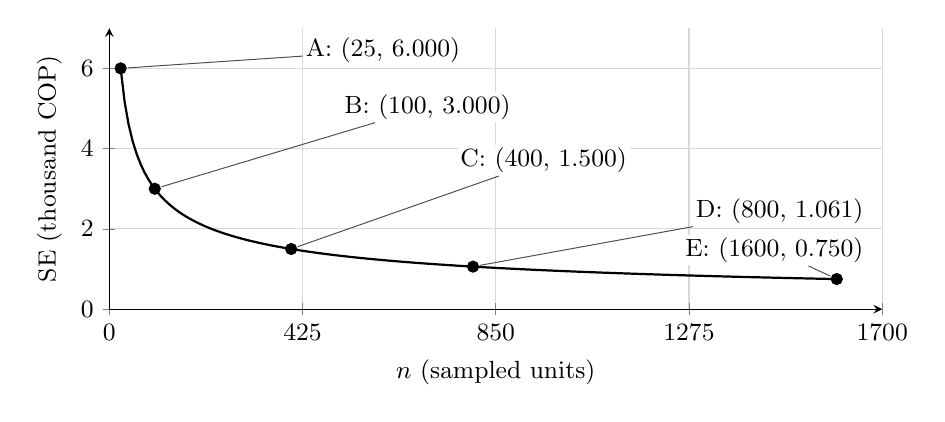
\begin{tikzpicture}\begin{axis}[relation,xlabel={$\CtwoSize{n}$ (sampled units)},ylabel={$\CtwoSE{\mathrm{SE}}$ (thousand COP)},xmin=0,xmax=1700,ymin=0,ymax=7,xtick={0,425,850,1275,1700}]
\addplot[thick,CthreeSELine,domain=25:1600,samples=180] {30/sqrt(x)};
\addplot[CthreeSELine,only marks,mark=*,mark size=2pt] coordinates {(25.000000000,6.000000000) (100.000000000,3.000000000) (400.000000000,1.500000000) (800.000000000,1.060660172) (1600.000000000,0.750000000)};
\PointLabel{A}{25.000000000,6.000000000}{25}{6.000}{0.25}{0.92}{west}
\PointLabel{B}{100.000000000,3.000000000}{100}{3.000}{0.3}{0.72}{west}
\PointLabel{C}{400.000000000,1.500000000}{400}{1.500}{0.45}{0.53}{west}
\PointLabel{D}{800.000000000,1.060660172}{800}{1.061}{0.98}{0.35}{east}
\PointLabel{E}{1600.000000000,0.750000000}{1600}{0.750}{0.98}{0.21}{east}
\end{axis}\end{tikzpicture}
\end{column}\begin{column}{.30\textwidth}\small $\CtwoSE{\mathrm{SE}}=\CtwoSD{30}/\sqrt{\CtwoSize{n}}$.\par\par\medskip As sample size increases, SE decreases as $1/\sqrt n$. Quadrupling $n$ halves SE.\end{column}\end{columns}
\end{frame}

% Source: Classroom :157--167; colored treatments Practice :18--29.
\begin{frame}[t]{Margin of error vs sample size}
\let\XRole\CtwoSize\let\YRole\CtwoMoE
\begin{columns}[T,onlytextwidth]\begin{column}{.68\textwidth}
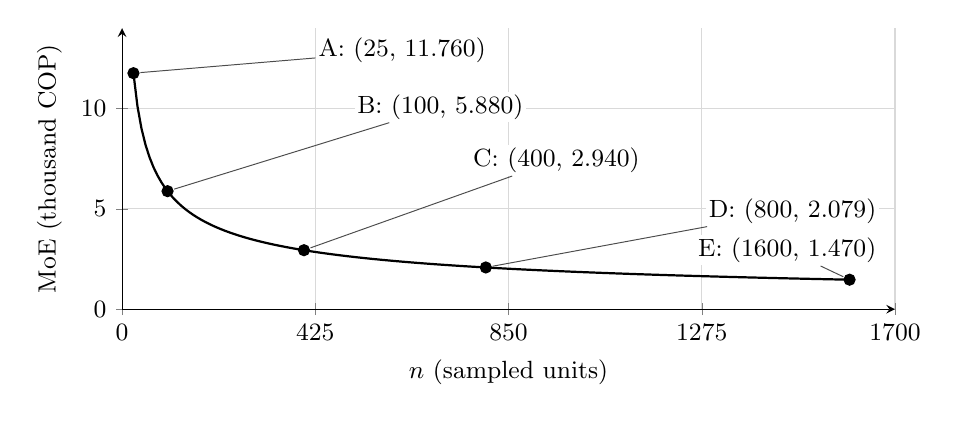
\begin{tikzpicture}\begin{axis}[relation,xlabel={$\CtwoSize{n}$ (sampled units)},ylabel={$\CtwoMoE{\mathrm{MoE}}$ (thousand COP)},xmin=0,xmax=1700,ymin=0,ymax=14,xtick={0,425,850,1275,1700}]
\addplot[thick,CthreeMoELine,domain=25:1600,samples=180] {1.960*30/sqrt(x)};
\addplot[CthreeMoELine,only marks,mark=*,mark size=2pt] coordinates {(25.000000000,11.760000000) (100.000000000,5.880000000) (400.000000000,2.940000000) (800.000000000,2.078893937) (1600.000000000,1.470000000)};
\PointLabel{A}{25.000000000,11.760000000}{25}{11.760}{0.25}{0.92}{west}
\PointLabel{B}{100.000000000,5.880000000}{100}{5.880}{0.3}{0.72}{west}
\PointLabel{C}{400.000000000,2.940000000}{400}{2.940}{0.45}{0.53}{west}
\PointLabel{D}{800.000000000,2.078893937}{800}{2.079}{0.98}{0.35}{east}
\PointLabel{E}{1600.000000000,1.470000000}{1600}{1.470}{0.98}{0.21}{east}
\end{axis}\end{tikzpicture}
\end{column}\begin{column}{.30\textwidth}\small $\CtwoMoE{\mathrm{MoE}}=$\par $\CtwoCritical{1.960}\,\CtwoSE{\mathrm{SE}}$.\par $\CtwoSE{\mathrm{SE}}=\CtwoSD{30}/\sqrt{\CtwoSize{n}}$.\par\par\medskip Larger samples give narrower intervals and greater precision at the same 95\% confidence.\end{column}\end{columns}
\end{frame}

% Source: Classroom :171--178; colored treatments Practice :18--29.
\begin{frame}[t]{Margin of error vs standard error}
\let\XRole\CtwoSE\let\YRole\CtwoMoE
\begin{columns}[T,onlytextwidth]\begin{column}{.68\textwidth}
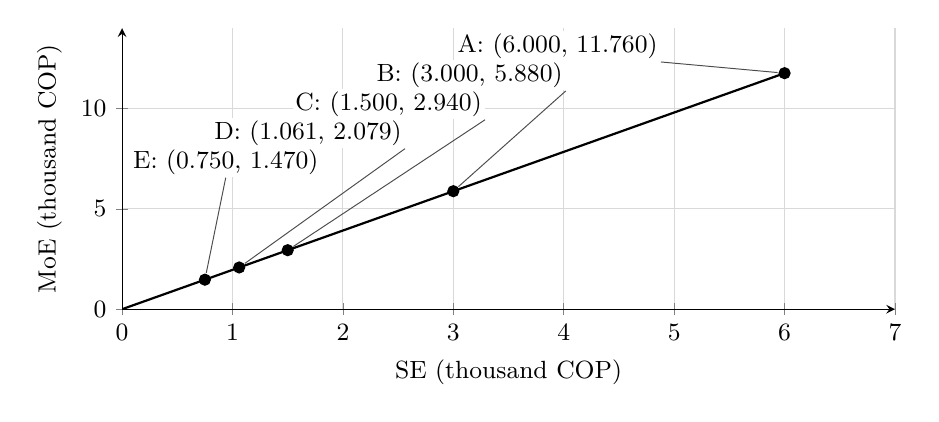
\begin{tikzpicture}\begin{axis}[relation,xlabel={$\CtwoSE{\mathrm{SE}}$ (thousand COP)},ylabel={$\CtwoMoE{\mathrm{MoE}}$ (thousand COP)},xmin=0,xmax=7,ymin=0,ymax=14]
\addplot[thick,CthreeMoELine,domain=0:6.0] {1.960*x};
\addplot[CthreeMoELine,only marks,mark=*,mark size=2pt] coordinates {(6.000000000,11.760000000) (3.000000000,5.880000000) (1.500000000,2.940000000) (1.060660172,2.078893937) (0.750000000,1.470000000)};
\def\guideStart{0.010}\def\guideStep{0.105}%
\def\guideSlope{1.960*7/14}\def\guideOffset{0.5147}%
\LinearGuideLabel{A}{6.000000000,11.760000000}{6.000}{11.760}{4}
\LinearGuideLabel{B}{3.000000000,5.880000000}{3.000}{5.880}{3}
\LinearGuideLabel{C}{1.500000000,2.940000000}{1.500}{2.940}{2}
\LinearGuideLabel[south east]{D}{1.060660172,2.078893937}{1.061}{2.079}{1}
\LinearGuideLabel[south]{E}{0.750000000,1.470000000}{0.750}{1.470}{0}
\end{axis}\end{tikzpicture}
\end{column}\begin{column}{.30\textwidth}\small $\CtwoMoE{\mathrm{MoE}}=$\par $\CtwoCritical{1.960}\CtwoSE{\mathrm{SE}}$.\par\par\medskip A line through the origin: the fixed critical value is its slope. SE and MoE decrease together as $1/\sqrt n$.\end{column}\end{columns}
\end{frame}

% Source: Classroom :182--193.
\begin{frame}[t]{The confidence interval stays centred at 84}

The \CtwoPoint{point estimate} centres the interval for the district mean $\CtwoMean{\mu}$.
\[
\CtwoEndpoint{\mathrm{CI}}=[\CtwoPoint{\bar x}-\CtwoMoE{\mathrm{MoE}},\;\CtwoPoint{\bar x}+\CtwoMoE{\mathrm{MoE}}]
\]
\visible<2->{At 95\% confidence: $\CtwoPoint{84}\pm\CtwoCritical{1.960}(\CtwoSD{30}/\sqrt{\CtwoSize{n}})$.}
\par\medskip
\visible<3->{\begin{tabular}{@{}l>{\raggedright\arraybackslash}p{.36\linewidth}>{\raggedright\arraybackslash}p{.43\linewidth}@{}}\toprule
Sample size & Centre $\pm$ margin & Interval (thousand COP)\\\midrule
$\CtwoSize{25}$&$\CtwoPoint{84}\pm\CtwoMoE{11.760}$&$\CtwoEndpoint{[72.240,95.760]}$\\
$\CtwoSize{400}$&$\CtwoPoint{84}\pm\CtwoMoE{2.940}$&$\CtwoEndpoint{[81.060,86.940]}$\\
$\CtwoSize{1600}$&$\CtwoPoint{84}\pm\CtwoMoE{1.470}$&$\CtwoEndpoint{[82.530,85.470]}$\\\bottomrule
\end{tabular}}

\end{frame}

% Source: Classroom :194--217.
\begin{frame}[t]{Explanatory confidence-interval comparison}
\centering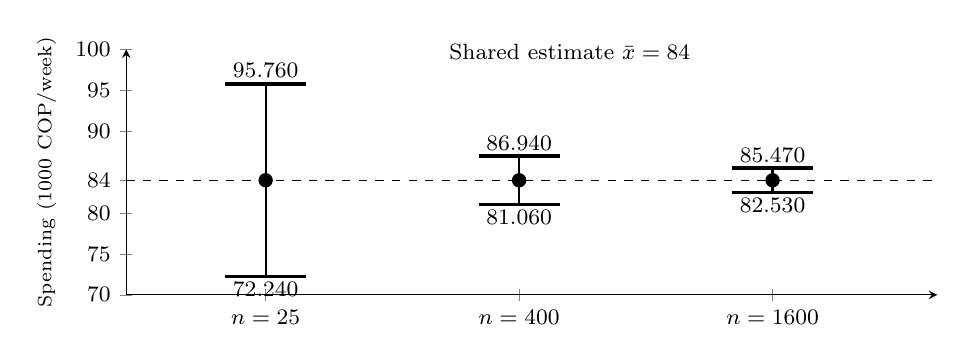
\begin{tikzpicture}\begin{axis}[
width=.98\linewidth,height=4.7cm,xmin=.45,xmax=3.65,ymin=70,ymax=100,
axis x line=bottom,axis y line=left,xtick={1,2,3},
xticklabels={$n=25$,$n=400$,$n=1600$},ytick={70,75,80,84,90,95,100},
tick label style={font=\footnotesize},label style={font=\footnotesize},
ylabel={\scriptsize Spending (1000 COP/week)},scaled ticks=false,clip=false]
\draw[dashed,EstimateLine] (axis cs:.45,84)--(axis cs:3.65,84);
\node[font=\footnotesize,anchor=south] at (axis cs:2.2,97.5) {Shared estimate $\CtwoPoint{\bar{x}}=\CtwoPoint{84}$};
\draw[CthreeMoELine,thick] (axis cs:1,72.240)--(axis cs:1,95.760);
\draw[CthreeMoELine,line width=1.3pt] (axis cs:0.84,72.240)--(axis cs:1.16,72.240)
(axis cs:0.84,95.760)--(axis cs:1.16,95.760);
\fill[EstimateLine] (axis cs:1,84) circle (2.6pt);
\node[font=\footnotesize,anchor=north,inner sep=2pt] at (axis cs:1,72.240) {$\CtwoEndpoint{72.240}$};
\node[font=\footnotesize,anchor=south,inner sep=2pt] at (axis cs:1,95.760) {$\CtwoEndpoint{95.760}$};
\draw[CthreeMoELine,thick] (axis cs:2,81.060)--(axis cs:2,86.940);
\draw[CthreeMoELine,line width=1.3pt] (axis cs:1.84,81.060)--(axis cs:2.16,81.060)
(axis cs:1.84,86.940)--(axis cs:2.16,86.940);
\fill[EstimateLine] (axis cs:2,84) circle (2.6pt);
\node[font=\footnotesize,anchor=north,inner sep=2pt] at (axis cs:2,81.060) {$\CtwoEndpoint{81.060}$};
\node[font=\footnotesize,anchor=south,inner sep=2pt] at (axis cs:2,86.940) {$\CtwoEndpoint{86.940}$};
\draw[CthreeMoELine,thick] (axis cs:3,82.530)--(axis cs:3,85.470);
\draw[CthreeMoELine,line width=1.3pt] (axis cs:2.84,82.530)--(axis cs:3.16,82.530)
(axis cs:2.84,85.470)--(axis cs:3.16,85.470);
\fill[EstimateLine] (axis cs:3,84) circle (2.6pt);
\node[font=\footnotesize,anchor=north,inner sep=2pt] at (axis cs:3,82.530) {$\CtwoEndpoint{82.530}$};
\node[font=\footnotesize,anchor=south,inner sep=2pt] at (axis cs:3,85.470) {$\CtwoEndpoint{85.470}$};
\end{axis}\end{tikzpicture}
\raggedright\small Same estimate and 95\% confidence; larger samples reduce SE and MoE, producing narrower intervals and greater precision.
\end{frame}

\section{Task 2}
% Source: Classroom :114--123, :219--220.
\begin{frame}[t]{Task 2: Vary confidence}

Keep $\CtwoSize{n}=\CtwoSize{100}$ and $\CtwoSD{\sigma}=\CtwoSD{30}$ thousand COP fixed.
\par\medskip
\begin{tabular}{@{}l*{5}{>{\centering\arraybackslash}p{.15\linewidth}}@{}}\toprule
ID&A&B&C&D&E\\\midrule
$\CtwoConfidence{C}$ (\%)&\CtwoConfidence{80}&\CtwoConfidence{90}&\CtwoConfidence{95}&\CtwoConfidence{99}&\CtwoConfidence{99.9}\\
$\CtwoCritical{z^*}$&\CtwoCritical{1.282}&\CtwoCritical{1.645}&\CtwoCritical{1.960}&\CtwoCritical{2.576}&\CtwoCritical{3.291}\\\bottomrule\end{tabular}
\par\medskip
\textbf{Calculate} fixed SE and the MoE for each supplied pair.\par
\textbf{Draw} confidence vs MoE, critical value vs MoE, and confidence vs critical value; label A--E with coordinates.
\par\medskip
\visible<2->{The \CtwoCritical{critical value} is a unitless normal cutoff. \CtwoConfidence{Confidence} is the nominal long-run percentage of intervals covering $\CtwoMean{\mu}$ under the model.}

\end{frame}

% Source: Classroom :219--220; definitions :94--108.
\begin{frame}[t]{Task 2: Fixed SE, changing multiplier}

\[
\CtwoSE{\mathrm{SE}}=\frac{\CtwoSD{\sigma}}{\sqrt{\CtwoSize{n}}}
\visible<2->{=\frac{\CtwoSD{30}}{\sqrt{\CtwoSize{100}}}=\CtwoSE{3.000}}
\]
\visible<3->{\[
\CtwoMoE{\mathrm{MoE}}=\CtwoCritical{z^*}\CtwoSE{\mathrm{SE}}=\CtwoCritical{z^*}(\CtwoSE{3.000})
\]}
\par\medskip
\visible<4->{For A: $\CtwoMoE{\mathrm{MoE}}=\CtwoCritical{1.282}(\CtwoSE{3.000})=\CtwoMoE{3.846}$ thousand COP.}
\par\medskip
\visible<5->{SE stays fixed because neither population SD nor sample size changes. The confidence choice changes the multiplier and therefore the margin.}

\end{frame}

% Source: Classroom :220.
\begin{frame}[t]{Task 2: Calculate all five margins}
\begin{tabular}{@{}lcc>{\raggedright\arraybackslash}p{.50\linewidth}@{}}\toprule ID&$\CtwoConfidence{C}$ (\%)&$\CtwoCritical{z^*}$&$\CtwoMoE{\mathrm{MoE}}=\CtwoCritical{z^*}(\CtwoSE{3.000})$\\\midrule
A & $\CtwoConfidence{80}$ & $\CtwoCritical{1.282}$ & $\visible<2->{\CtwoCritical{1.282}(\CtwoSE{3.000})=\CtwoMoE{3.846}}$\\
B & $\CtwoConfidence{90}$ & $\CtwoCritical{1.645}$ & $\visible<3->{\CtwoCritical{1.645}(\CtwoSE{3.000})=\CtwoMoE{4.935}}$\\
C & $\CtwoConfidence{95}$ & $\CtwoCritical{1.960}$ & $\visible<4->{\CtwoCritical{1.960}(\CtwoSE{3.000})=\CtwoMoE{5.880}}$\\
D & $\CtwoConfidence{99}$ & $\CtwoCritical{2.576}$ & $\visible<5->{\CtwoCritical{2.576}(\CtwoSE{3.000})=\CtwoMoE{7.728}}$\\
E & $\CtwoConfidence{99.9}$ & $\CtwoCritical{3.291}$ & $\visible<6->{\CtwoCritical{3.291}(\CtwoSE{3.000})=\CtwoMoE{9.873}}$\\\bottomrule\end{tabular}\par\medskip\par MoE: thousand COP; critical values: unitless.
\end{frame}

% Source: Classroom :222--232; colored treatments Practice :18--29.
\begin{frame}[t]{Confidence level vs margin of error}
\let\XRole\CtwoMoE\let\YRole\CtwoConfidence
\begin{columns}[T,onlytextwidth]\begin{column}{.68\textwidth}
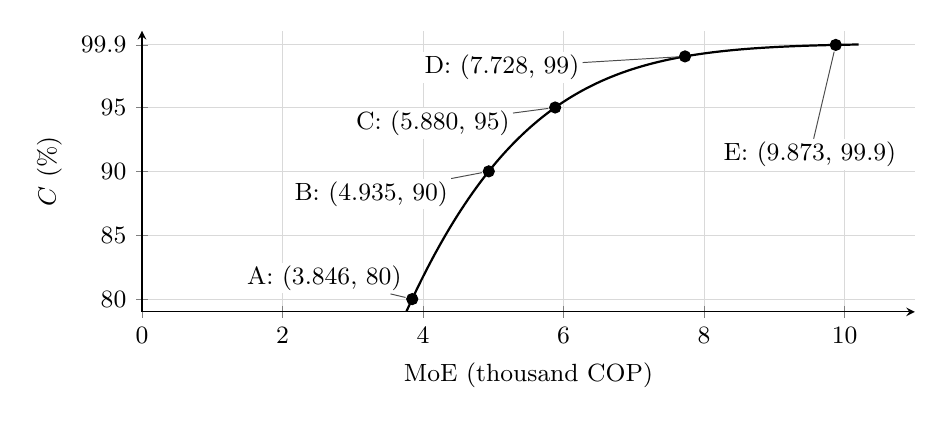
\begin{tikzpicture}\begin{axis}[relation,xlabel={$\CtwoMoE{\mathrm{MoE}}$ (thousand COP)},ylabel={$\CtwoConfidence{C}$ (\%)},xmin=0,xmax=11,ymin=79,ymax=101,ytick={80,85,90,95,99.9}]
\addplot[thick,CthreeConfidenceLine] coordinates {(3.600000000,76.986065956) (3.636666667,77.457267281) (3.673333333,77.921538814) (3.710000000,78.378914140) (3.746666667,78.829428390) (3.783333333,79.273118204) (3.820000000,79.710021689) (3.856666667,80.140178381) (3.893333333,80.563629207) (3.930000000,80.980416441) (3.966666667,81.390583669) (4.003333333,81.794175746) (4.040000000,82.191238757) (4.076666667,82.581819974) (4.113333333,82.965967820) (4.150000000,83.343731826) (4.186666667,83.715162592) (4.223333333,84.080311743) (4.260000000,84.439231895) (4.296666667,84.791976609) (4.333333333,85.138600354) (4.370000000,85.479158469) (4.406666667,85.813707116) (4.443333333,86.142303250) (4.480000000,86.465004571) (4.516666667,86.781869494) (4.553333333,87.092957100) (4.590000000,87.398327107) (4.626666667,87.698039826) (4.663333333,87.992156125) (4.700000000,88.280737392) (4.736666667,88.563845498) (4.773333333,88.841542760) (4.810000000,89.113891904) (4.846666667,89.380956033) (4.883333333,89.642798585) (4.920000000,89.899483305) (4.956666667,90.151074208) (4.993333333,90.397635545) (5.030000000,90.639231769) (5.066666667,90.875927504) (5.103333333,91.107787513) (5.140000000,91.334876665) (5.176666667,91.557259905) (5.213333333,91.775002224) (5.250000000,91.988168627) (5.286666667,92.196824108) (5.323333333,92.401033617) (5.360000000,92.600862035) (5.396666667,92.796374145) (5.433333333,92.987634608) (5.470000000,93.174707932) (5.506666667,93.357658453) (5.543333333,93.536550307) (5.580000000,93.711447404) (5.616666667,93.882413408) (5.653333333,94.049511715) (5.690000000,94.212805427) (5.726666667,94.372357332) (5.763333333,94.528229888) (5.800000000,94.680485196) (5.836666667,94.829184985) (5.873333333,94.974390591) (5.910000000,95.116162944) (5.946666667,95.254562542) (5.983333333,95.389649443) (6.020000000,95.521483244) (6.056666667,95.650123066) (6.093333333,95.775627542) (6.130000000,95.898054799) (6.166666667,96.017462450) (6.203333333,96.133907575) (6.240000000,96.247446713) (6.276666667,96.358135850) (6.313333333,96.466030405) (6.350000000,96.571185226) (6.386666667,96.673654573) (6.423333333,96.773492113) (6.460000000,96.870750912) (6.496666667,96.965483425) (6.533333333,97.057741490) (6.570000000,97.147576318) (6.606666667,97.235038493) (6.643333333,97.320177959) (6.680000000,97.403044022) (6.716666667,97.483685338) (6.753333333,97.562149914) (6.790000000,97.638485104) (6.826666667,97.712737601) (6.863333333,97.784953441) (6.900000000,97.855177996) (6.936666667,97.923455973) (6.973333333,97.989831414) (7.010000000,98.054347695) (7.046666667,98.117047523) (7.083333333,98.177972938) (7.120000000,98.237165314) (7.156666667,98.294665358) (7.193333333,98.350513110) (7.230000000,98.404747948) (7.266666667,98.457408586) (7.303333333,98.508533080) (7.340000000,98.558158826) (7.376666667,98.606322564) (7.413333333,98.653060386) (7.450000000,98.698407731) (7.486666667,98.742399394) (7.523333333,98.785069530) (7.560000000,98.826451657) (7.596666667,98.866578658) (7.633333333,98.905482789) (7.670000000,98.943195683) (7.706666667,98.979748356) (7.743333333,99.015171209) (7.780000000,99.049494036) (7.816666667,99.082746030) (7.853333333,99.114955789) (7.890000000,99.146151318) (7.926666667,99.176360042) (7.963333333,99.205608807) (8.000000000,99.233923886) (8.036666667,99.261330993) (8.073333333,99.287855279) (8.110000000,99.313521347) (8.146666667,99.338353257) (8.183333333,99.362374529) (8.220000000,99.385608156) (8.256666667,99.408076609) (8.293333333,99.429801841) (8.330000000,99.450805300) (8.366666667,99.471107932) (8.403333333,99.490730189) (8.440000000,99.509692041) (8.476666667,99.528012976) (8.513333333,99.545712013) (8.550000000,99.562807709) (8.586666667,99.579318164) (8.623333333,99.595261032) (8.660000000,99.610653524) (8.696666667,99.625512422) (8.733333333,99.639854079) (8.770000000,99.653694435) (8.806666667,99.667049015) (8.843333333,99.679932946) (8.880000000,99.692360958) (8.916666667,99.704347393) (8.953333333,99.715906214) (8.990000000,99.727051011) (9.026666667,99.737795010) (9.063333333,99.748151076) (9.100000000,99.758131727) (9.136666667,99.767749133) (9.173333333,99.777015132) (9.210000000,99.785941229) (9.246666667,99.794538609) (9.283333333,99.802818141) (9.320000000,99.810790383) (9.356666667,99.818465596) (9.393333333,99.825853741) (9.430000000,99.832964493) (9.466666667,99.839807245) (9.503333333,99.846391114) (9.540000000,99.852724948) (9.576666667,99.858817332) (9.613333333,99.864676596) (9.650000000,99.870310818) (9.686666667,99.875727832) (9.723333333,99.880935234) (9.760000000,99.885940387) (9.796666667,99.890750427) (9.833333333,99.895372271) (9.870000000,99.899812617) (9.906666667,99.904077957) (9.943333333,99.908174575) (9.980000000,99.912108558) (10.016666667,99.915885798) (10.053333333,99.919511999) (10.090000000,99.922992681) (10.126666667,99.926333183) (10.163333333,99.929538672) (10.200000000,99.932614147)};
\addplot[CthreeConfidenceLine,only marks,mark=*,mark size=2pt] coordinates {(3.846000000,80.000000000) (4.935000000,90.000000000) (5.880000000,95.000000000) (7.728000000,99.000000000) (9.873000000,99.900000000)};
\PointLabel{A}{3.846000000,80.000000000}{3.846}{80}{0.34}{0.12}{east}
\PointLabel{B}{4.935000000,90.000000000}{4.935}{90}{0.40}{0.42}{east}
\PointLabel{C}{5.880000000,95.000000000}{5.880}{95}{0.48}{0.67}{east}
\PointLabel{D}{7.728000000,99.000000000}{7.728}{99}{0.57}{0.87}{east}
\PointLabel{E}{9.873000000,99.900000000}{9.873}{99.9}{0.98}{0.56}{east}
\end{axis}\end{tikzpicture}
\end{column}\begin{column}{.30\textwidth}\small Fixed $\CtwoSE{\mathrm{SE}}=\CtwoSE{3.000}$.\par\par\medskip Higher confidence requires a larger margin: intervals widen and precision decreases.\par\par\medskip Curve: theoretical normal coverage. A--E: nominal confidence.\end{column}\end{columns}
\end{frame}

% Source: Classroom :236--246; colored treatments Practice :18--29.
\begin{frame}[t]{Critical value vs margin of error}
\let\XRole\CtwoMoE\let\YRole\CtwoCritical
\begin{columns}[T,onlytextwidth]\begin{column}{.68\textwidth}
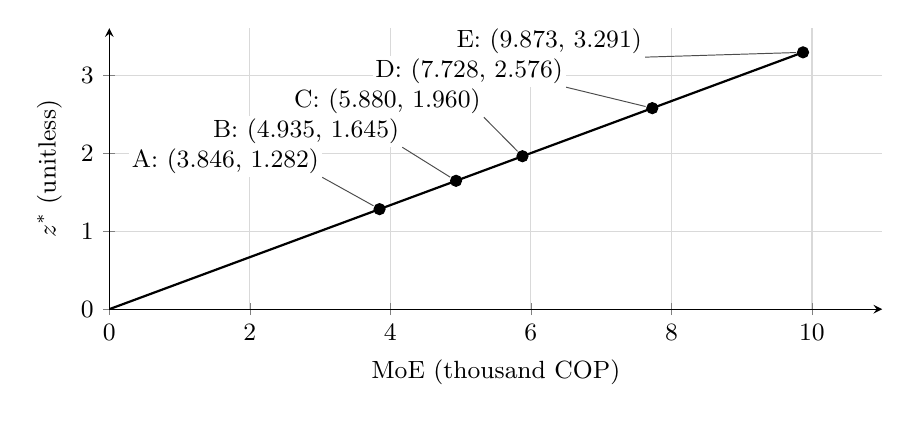
\begin{tikzpicture}\begin{axis}[relation,xlabel={$\CtwoMoE{\mathrm{MoE}}$ (thousand COP)},ylabel={$\CtwoCritical{z^*}$ (unitless)},xmin=0,xmax=11,ymin=0,ymax=3.6,ytick={0,1,2,3}]
\addplot[thick,CthreeCriticalLine,domain=0:9.873] {x/3.0};
\addplot[CthreeCriticalLine,only marks,mark=*,mark size=2pt] coordinates {(3.846000000,1.282000000) (4.935000000,1.645000000) (5.880000000,1.960000000) (7.728000000,2.576000000) (9.873000000,3.291000000)};
\def\guideStart{0.025}\def\guideStep{0.105}%
\def\guideSlope{11/(3*3.6)}\def\guideOffset{0.50}%
\LinearGuideLabel{A}{3.846000000,1.282000000}{3.846}{1.282}{0}
\LinearGuideLabel{B}{4.935000000,1.645000000}{4.935}{1.645}{1}
\LinearGuideLabel{C}{5.880000000,1.960000000}{5.880}{1.960}{2}
\LinearGuideLabel{D}{7.728000000,2.576000000}{7.728}{2.576}{3}
\LinearGuideLabel{E}{9.873000000,3.291000000}{9.873}{3.291}{4}
\end{axis}\end{tikzpicture}
\end{column}\begin{column}{.30\textwidth}\small $\CtwoCritical{z^*}=\CtwoMoE{\mathrm{MoE}}/\CtwoSE{3.000}$.\par\par\medskip At fixed SE, MoE increases with $z^*$. The relationship is linear through the origin.\end{column}\end{columns}
\end{frame}

% Source: Classroom :250--260; colored treatments Practice :18--29.
\begin{frame}[t]{Confidence level vs critical value}
\let\XRole\CtwoCritical\let\YRole\CtwoConfidence
\begin{columns}[T,onlytextwidth]\begin{column}{.68\textwidth}
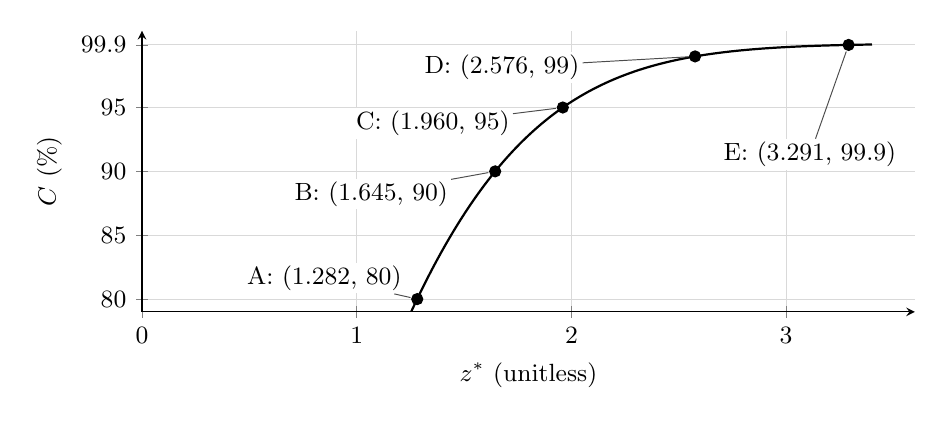
\begin{tikzpicture}\begin{axis}[relation,xlabel={$\CtwoCritical{z^*}$ (unitless)},ylabel={$\CtwoConfidence{C}$ (\%)},xmin=0,xmax=3.6,ymin=79,ymax=101,xtick={0,1,2,3},ytick={80,85,90,95,99.9}]
\addplot[thick,CthreeConfidenceLine] coordinates {(1.200000000,76.986065956) (1.212222222,77.457267281) (1.224444444,77.921538814) (1.236666667,78.378914140) (1.248888889,78.829428390) (1.261111111,79.273118204) (1.273333333,79.710021689) (1.285555556,80.140178381) (1.297777778,80.563629207) (1.310000000,80.980416441) (1.322222222,81.390583669) (1.334444444,81.794175746) (1.346666667,82.191238757) (1.358888889,82.581819974) (1.371111111,82.965967820) (1.383333333,83.343731826) (1.395555556,83.715162592) (1.407777778,84.080311743) (1.420000000,84.439231895) (1.432222222,84.791976609) (1.444444444,85.138600354) (1.456666667,85.479158469) (1.468888889,85.813707116) (1.481111111,86.142303250) (1.493333333,86.465004571) (1.505555556,86.781869494) (1.517777778,87.092957100) (1.530000000,87.398327107) (1.542222222,87.698039826) (1.554444444,87.992156125) (1.566666667,88.280737392) (1.578888889,88.563845498) (1.591111111,88.841542760) (1.603333333,89.113891904) (1.615555556,89.380956033) (1.627777778,89.642798585) (1.640000000,89.899483305) (1.652222222,90.151074208) (1.664444444,90.397635545) (1.676666667,90.639231769) (1.688888889,90.875927504) (1.701111111,91.107787513) (1.713333333,91.334876665) (1.725555556,91.557259905) (1.737777778,91.775002224) (1.750000000,91.988168627) (1.762222222,92.196824108) (1.774444444,92.401033617) (1.786666667,92.600862035) (1.798888889,92.796374145) (1.811111111,92.987634608) (1.823333333,93.174707932) (1.835555556,93.357658453) (1.847777778,93.536550307) (1.860000000,93.711447404) (1.872222222,93.882413408) (1.884444444,94.049511715) (1.896666667,94.212805427) (1.908888889,94.372357332) (1.921111111,94.528229888) (1.933333333,94.680485196) (1.945555556,94.829184985) (1.957777778,94.974390591) (1.970000000,95.116162944) (1.982222222,95.254562542) (1.994444444,95.389649443) (2.006666667,95.521483244) (2.018888889,95.650123066) (2.031111111,95.775627542) (2.043333333,95.898054799) (2.055555556,96.017462450) (2.067777778,96.133907575) (2.080000000,96.247446713) (2.092222222,96.358135850) (2.104444444,96.466030405) (2.116666667,96.571185226) (2.128888889,96.673654573) (2.141111111,96.773492113) (2.153333333,96.870750912) (2.165555556,96.965483425) (2.177777778,97.057741490) (2.190000000,97.147576318) (2.202222222,97.235038493) (2.214444444,97.320177959) (2.226666667,97.403044022) (2.238888889,97.483685338) (2.251111111,97.562149914) (2.263333333,97.638485104) (2.275555556,97.712737601) (2.287777778,97.784953441) (2.300000000,97.855177996) (2.312222222,97.923455973) (2.324444444,97.989831414) (2.336666667,98.054347695) (2.348888889,98.117047523) (2.361111111,98.177972938) (2.373333333,98.237165314) (2.385555556,98.294665358) (2.397777778,98.350513110) (2.410000000,98.404747948) (2.422222222,98.457408586) (2.434444444,98.508533080) (2.446666667,98.558158826) (2.458888889,98.606322564) (2.471111111,98.653060386) (2.483333333,98.698407731) (2.495555556,98.742399394) (2.507777778,98.785069530) (2.520000000,98.826451657) (2.532222222,98.866578658) (2.544444444,98.905482789) (2.556666667,98.943195683) (2.568888889,98.979748356) (2.581111111,99.015171209) (2.593333333,99.049494036) (2.605555556,99.082746030) (2.617777778,99.114955789) (2.630000000,99.146151318) (2.642222222,99.176360042) (2.654444444,99.205608807) (2.666666667,99.233923886) (2.678888889,99.261330993) (2.691111111,99.287855279) (2.703333333,99.313521347) (2.715555556,99.338353257) (2.727777778,99.362374529) (2.740000000,99.385608156) (2.752222222,99.408076609) (2.764444444,99.429801841) (2.776666667,99.450805300) (2.788888889,99.471107932) (2.801111111,99.490730189) (2.813333333,99.509692041) (2.825555556,99.528012976) (2.837777778,99.545712013) (2.850000000,99.562807709) (2.862222222,99.579318164) (2.874444444,99.595261032) (2.886666667,99.610653524) (2.898888889,99.625512422) (2.911111111,99.639854079) (2.923333333,99.653694435) (2.935555556,99.667049015) (2.947777778,99.679932946) (2.960000000,99.692360958) (2.972222222,99.704347393) (2.984444444,99.715906214) (2.996666667,99.727051011) (3.008888889,99.737795010) (3.021111111,99.748151076) (3.033333333,99.758131727) (3.045555556,99.767749133) (3.057777778,99.777015132) (3.070000000,99.785941229) (3.082222222,99.794538609) (3.094444444,99.802818141) (3.106666667,99.810790383) (3.118888889,99.818465596) (3.131111111,99.825853741) (3.143333333,99.832964493) (3.155555556,99.839807245) (3.167777778,99.846391114) (3.180000000,99.852724948) (3.192222222,99.858817332) (3.204444444,99.864676596) (3.216666667,99.870310818) (3.228888889,99.875727832) (3.241111111,99.880935234) (3.253333333,99.885940387) (3.265555556,99.890750427) (3.277777778,99.895372271) (3.290000000,99.899812617) (3.302222222,99.904077957) (3.314444444,99.908174575) (3.326666667,99.912108558) (3.338888889,99.915885798) (3.351111111,99.919511999) (3.363333333,99.922992681) (3.375555556,99.926333183) (3.387777778,99.929538672) (3.400000000,99.932614147)};
\addplot[CthreeConfidenceLine,only marks,mark=*,mark size=2pt] coordinates {(1.282000000,80.000000000) (1.645000000,90.000000000) (1.960000000,95.000000000) (2.576000000,99.000000000) (3.291000000,99.900000000)};
\PointLabel{A}{1.282000000,80.000000000}{1.282}{80}{0.34}{0.12}{east}
\PointLabel{B}{1.645000000,90.000000000}{1.645}{90}{0.40}{0.42}{east}
\PointLabel{C}{1.960000000,95.000000000}{1.960}{95}{0.48}{0.67}{east}
\PointLabel{D}{2.576000000,99.000000000}{2.576}{99}{0.57}{0.87}{east}
\PointLabel{E}{3.291000000,99.900000000}{3.291}{99.9}{0.98}{0.56}{east}
\end{axis}\end{tikzpicture}
\end{column}\begin{column}{.30\textwidth}\small Higher confidence requires a larger $\CtwoCritical{z^*}$.\par\par\medskip Both normal cutoffs move outward, enclosing a larger central area.\par\par\medskip Curve: theoretical coverage. A--E: nominal confidence.\end{column}\end{columns}
\end{frame}

% Source: Classroom :222--260 curve coordinates; Practice :89--93 and registered theoretical-coverage meaning.
% Source: registered theoretical coverage; Classroom normal curve data.
\begin{frame}[t]{Reading the confidence curves}
The supplied $\CtwoCritical{z^*}$ values are rounded to three decimals.
\par\medskip
\[
\HLCumulativeProbability{C_{\rm normal}}=2\HLCumulativeProbability{\Phi}(\CtwoCritical{z^*})-1
\]
\par\medskip
\par\medskip\par The curves use normal coverage; the plotted markers use nominal percentages. The small differences come from rounding the cutoffs.


\end{frame}
\begin{frame}[t]{Nominal confidence and theoretical normal coverage}

The supplied $\CtwoCritical{z^*}$ values are rounded to three decimals.

\small
\begin{tabular}{@{}lcc>{\raggedright\arraybackslash}p{.50\linewidth}@{}}\toprule
ID&Nominal $\CtwoConfidence{C}$&$\CtwoCritical{z^*}$&$100[2\Phi(z^*)-1]$\\\midrule
A&\CtwoConfidence{80\%}&\CtwoCritical{1.282}&\HLCumulativeProbability{80.01574\%}\\
B&\CtwoConfidence{90\%}&\CtwoCritical{1.645}&\HLCumulativeProbability{90.00302\%}\\
C&\CtwoConfidence{95\%}&\CtwoCritical{1.960}&\HLCumulativeProbability{95.00042\%}\\
D&\CtwoConfidence{99\%}&\CtwoCritical{2.576}&\HLCumulativeProbability{99.00049\%}\\
E&\CtwoConfidence{99.9\%}&\CtwoCritical{3.291}&\HLCumulativeProbability{99.90017\%}\\\bottomrule\end{tabular}
\end{frame}

% Source: Classroom :71--84, :263--266; practice graph style :50--78.
\begin{frame}[t]{Standard normal illustration: case A}
$Z\sim N(0,1)$: the cutoffs enclose the central region.
\begin{center}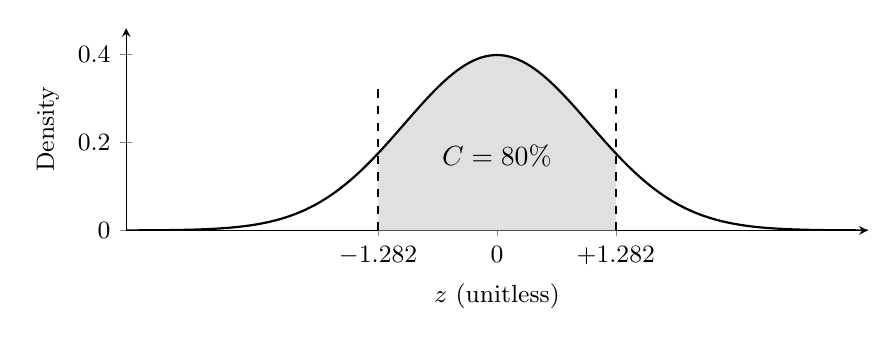
\begin{tikzpicture}\begin{axis}[
width=11cm,height=4.15cm,xmin=-4,xmax=4,ymin=0,ymax=.46,
enlargelimits=false,axis lines=left,xtick={-1.282,0,1.282},
xticklabels={$\CtwoCritical{-1.282}$,0,$\CtwoCritical{+1.282}$},ytick={0,.2,.4},
xlabel={$z$ (unitless)},ylabel={Density},tick label style={font=\small},label style={font=\small}]
\addplot[draw=none,fill=CthreeConfidenceFill,domain=-1.282:1.282,samples=161] {exp(-x*x/2)/sqrt(2*pi)}\closedcycle;
\addplot[black,thick,domain=-4:4,samples=201] {exp(-x*x/2)/sqrt(2*pi)};
\draw[CthreeCriticalLine,thick,dashed] (axis cs:-1.282,0)--(axis cs:-1.282,.33) (axis cs:1.282,0)--(axis cs:1.282,.33);
\node at (axis cs:0,.17) {$\CtwoConfidence{C=80\%}$};
\end{axis}\end{tikzpicture}\end{center}
\small Nominal $\CtwoConfidence{C}=\CtwoConfidence{80\%}$; shaded theoretical normal coverage $\HLCumulativeProbability{C_{\rm normal}}\approx\HLCumulativeProbability{80.01574\%}$.

\end{frame}

% Source: Classroom :71--84, :263--266; practice graph style :50--78.
\begin{frame}[t]{Standard normal illustration: case C}
$Z\sim N(0,1)$: the cutoffs enclose the central region.
\begin{center}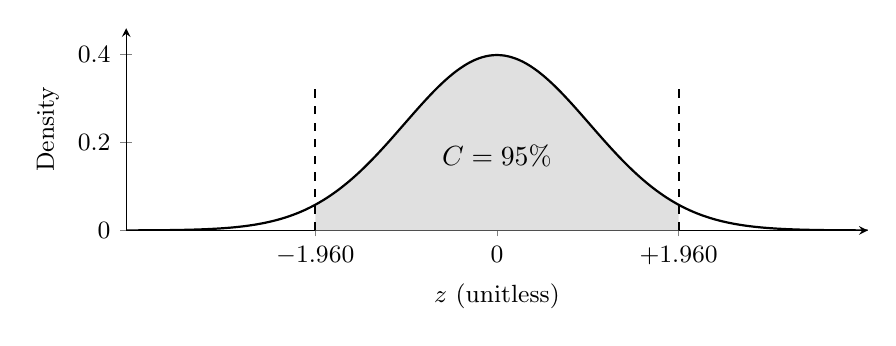
\begin{tikzpicture}\begin{axis}[
width=11cm,height=4.15cm,xmin=-4,xmax=4,ymin=0,ymax=.46,
enlargelimits=false,axis lines=left,xtick={-1.960,0,1.960},
xticklabels={$\CtwoCritical{-1.960}$,0,$\CtwoCritical{+1.960}$},ytick={0,.2,.4},
xlabel={$z$ (unitless)},ylabel={Density},tick label style={font=\small},label style={font=\small}]
\addplot[draw=none,fill=CthreeConfidenceFill,domain=-1.960:1.960,samples=161] {exp(-x*x/2)/sqrt(2*pi)}\closedcycle;
\addplot[black,thick,domain=-4:4,samples=201] {exp(-x*x/2)/sqrt(2*pi)};
\draw[CthreeCriticalLine,thick,dashed] (axis cs:-1.960,0)--(axis cs:-1.960,.33) (axis cs:1.960,0)--(axis cs:1.960,.33);
\node at (axis cs:0,.17) {$\CtwoConfidence{C=95\%}$};
\end{axis}\end{tikzpicture}\end{center}
\small Nominal $\CtwoConfidence{C}=\CtwoConfidence{95\%}$; shaded theoretical normal coverage $\HLCumulativeProbability{C_{\rm normal}}\approx\HLCumulativeProbability{95.00042\%}$.

\end{frame}

% Source: Classroom :71--84, :263--266; practice graph style :50--78.
\begin{frame}[t]{Standard normal illustration: case E}
$Z\sim N(0,1)$: the cutoffs enclose the central region.
\begin{center}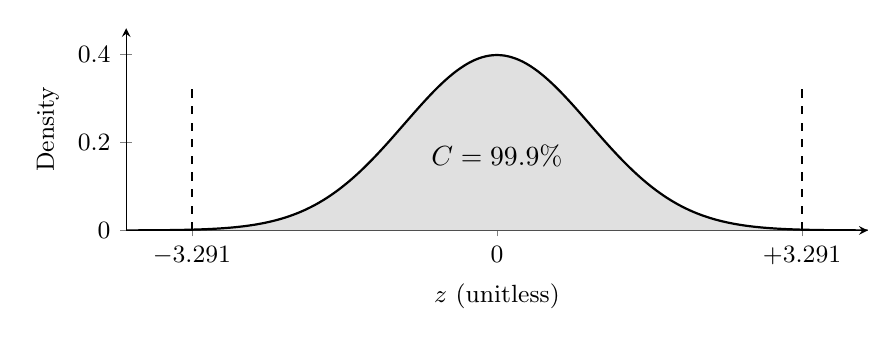
\begin{tikzpicture}\begin{axis}[
width=11cm,height=4.15cm,xmin=-4,xmax=4,ymin=0,ymax=.46,
enlargelimits=false,axis lines=left,xtick={-3.291,0,3.291},
xticklabels={$\CtwoCritical{-3.291}$,0,$\CtwoCritical{+3.291}$},ytick={0,.2,.4},
xlabel={$z$ (unitless)},ylabel={Density},tick label style={font=\small},label style={font=\small}]
\addplot[draw=none,fill=CthreeConfidenceFill,domain=-3.291:3.291,samples=161] {exp(-x*x/2)/sqrt(2*pi)}\closedcycle;
\addplot[black,thick,domain=-4:4,samples=201] {exp(-x*x/2)/sqrt(2*pi)};
\draw[CthreeCriticalLine,thick,dashed] (axis cs:-3.291,0)--(axis cs:-3.291,.33) (axis cs:3.291,0)--(axis cs:3.291,.33);
\node at (axis cs:0,.17) {$\CtwoConfidence{C=99.9\%}$};
\end{axis}\end{tikzpicture}\end{center}
\small Nominal $\CtwoConfidence{C}=\CtwoConfidence{99.9\%}$; shaded theoretical normal coverage $\HLCumulativeProbability{C_{\rm normal}}\approx\HLCumulativeProbability{99.90017\%}$.

\end{frame}

\section{Synthesis}
% Source: Classroom :179--180, :259--260; criterion and definitions :89--108.
\begin{frame}[t]{What changes, and what stays fixed?}

\textbf{Task 1: same confidence, more observations.}\par
$\CtwoSE{\mathrm{SE}}\sim\CtwoMoE{\mathrm{MoE}}\sim1/\sqrt{\CtwoSize{n}}$. Larger samples give narrower intervals and greater precision at the same 95\% confidence.
\par\medskip
\visible<2->{\textbf{Task 2: same SE, greater confidence.}\par
Higher $\CtwoConfidence{C}$ requires a larger $\CtwoCritical{z^*}$, producing a larger $\CtwoMoE{\mathrm{MoE}}$, wider intervals, and lower precision.}
\par\medskip
\visible<3->{\textbf{The components work together.}\par
The $\CtwoPoint{84}$ thousand COP point estimate supplies the centre; critical value and SE determine the margin. Confidence describes the procedure's long-run reliability under the model assumptions.}

\end{frame}

\end{document}

